%\documentstyle[epsf,twocolumn]{jarticle}       %LaTeX2e仕様
\documentclass[twocolumn]{jarticle}     %pLaTeX2e仕様(platex.exeの場合)
% \documentclass[onecolumn]{ujarticle}   %pLaTeX2e仕様(uplatex.exeの場合)
%%%%%%%%%%%%%%%%%%%%%%%%%%%%%%%%%%%%%%%%%%%%%%%%%%%%%%%%%%%%%%
%%
%%  基本バージョン
%%
%%%%%%%%%%%%%%%%%%%%%%%%%%%%%%%%%%%%%%%%%%%%%%%%%%%%%%%%%%%%%%%%
\setlength{\topmargin}{-45pt}
%\setlength{\oddsidemargin}{0cm}
\setlength{\oddsidemargin}{-7.5mm}
%\setlength{\evensidemargin}{0cm}
\setlength{\textheight}{24.1cm}
%setlength{\textheight}{25cm}
\setlength{\textwidth}{17.4cm}
%\setlength{\textwidth}{172mm}
\setlength{\columnsep}{11mm}

%\kanjiskip=.07zw plus.5pt minus.5pt


% 【節が変わるごとに (1.1)(1.2) … (2.1)(2.2) と数式番号をつけるとき】
%\makeatletter
%\renewcommand{\theequation}{%
%\thesection.\arabic{equation}} %\@addtoreset{equation}{section}
%\makeatother

%\renewcommand{\arraystretch}{0.95} 行間の設定
%%%%%%%%%%%%%%%%%%%%%%%%%%%%%%%%%%%%%%%%%%%%%%%%%%%%%%%%
%\usepackage{graphicx}   %pLaTeX2e仕様(\documentstyle ->\documentclass)
\usepackage[dvipdfmx]{graphicx}
\usepackage{subcaption}
\usepackage{multirow}
\usepackage{amsmath}
\usepackage{url}
\usepackage{ulem}
\usepackage{algorithm}
\usepackage{algorithmic}
\usepackage{listings} %,jlisting} %日本語のコメントアウトをする場合jlistingが必要
%ここからソースコードの表示に関する設定
\lstset{
  basicstyle={\ttfamily},
  identifierstyle={\small},
  commentstyle={\smallitshape},
  keywordstyle={\small\bfseries},
  ndkeywordstyle={\small},
  stringstyle={\small\ttfamily},
  frame={tb},
  breaklines=true,
  columns=[l]{fullflexible},
  numbers=left,
  xrightmargin=0zw,
  xleftmargin=3zw,
  numberstyle={\scriptsize},
  stepnumber=1,
  numbersep=1zw,
  lineskip=-0.5ex
}
%%%%%%%%%%%%%%%%%%%%%%%%%%%%%%%%%%%%%%%%%%%%%%%%%%%%%%%%
\begin{document}

	%bibtex用の設定
	%\bibliographystyle{ujarticle}

	\twocolumn[
		\noindent
		\hspace{1em}
		2020 年 12 月 4 日
		ゼミ資料
		\hfill
		B4 杉山 竜弥
		\vspace{2mm}

		\hrule
		\begin{center}
			{\Large \bf 進捗報告}
		\end{center}
		\hrule
		\vspace{9mm}
	]

\section{今週やったこと}
\begin{itemize}
  \item GAの改良
\end{itemize}

\section{実験}

\subsection{問題}

後の順番で学習した個体が有利になるという欠点を修正するため, $w$と$\alpha$の訓練を分離した.
また適応度を正確にするため, 実際にサンプリングした$\alpha$とその時点の$w$で損失を計算した.
以下が改良したGAの手順.

\begin{enumerate}
  \item 一様乱数で初期個体生成
  \item 重み$w$を$\displaystyle \sum_{i \in P} \nabla_w \mathcal{L}_{\mathrm{train}}(w^*, \alpha^\mathrm{sampled}_i)$で更新
  \item 個体$\alpha$を$\displaystyle \nabla_\alpha \mathcal{L}_{\mathrm{valid}}(w^*, \alpha_i)$で更新
  \item 適応度$\displaystyle \mathcal{L}_{\mathrm{test}}(w, \alpha^\mathrm{sampled})$で個体$\alpha$を評価・選択
  \item 交叉・突然変異
  \item 収束するまで 2. に戻る
\end{enumerate}
($P$は個体群, $\alpha^\mathrm{sampled}$は隣接行列にサンプリングした$\alpha$)

\paragraph{$\alpha$の個体表現と交叉}
交叉は行列の同じ位置を参照する一様交叉を採用した.
遺伝子が実数なので, ブレンド交叉も試したが優良解が壊れやすいので導入するときはエリート保存戦略と組合せたい.

\subsection{実験設定}

\begin{table}[tb]
  \begin{center}
    \caption{モデルの設定}
    \begin{tabular}{|c|c|} \hline
      base model & VGG19 \\ \hline
      Optim($w$) & SGD(lr=0.001, momentum=0.9) \\ \hline
      Optim($\alpha$) & Adam(lr=0.003, $\beta$=(0.5, 0.999)) \\ \hline
      Loss & Cross Entropy Loss \\ \hline
      dataset & cifar10 \\ \hline
      pretrain & true \\ \hline
      batch size & 64 \\ \hline
      train size & 12500 \\ \hline
      valid size & 5000 \\ \hline
    \end{tabular}
    \label{tab:setting}
  \end{center}
\end{table}

\begin{table}[tb]
  \begin{center}
    \caption{GAの設定}
    \begin{tabular}{|c|c|} \hline
      個体数 & 10 \\ \hline
      世代数 & 20 \\ \hline \hline
      選択 & トーナメント \\ \hline
      サイズ & 2 \\ \hline \hline
      交叉 & 一様交叉 \\ \hline
      交叉率 & 0.5 \\ \hline \hline
      変異 & ガウス分布 \\ \hline
      変異率 & 0.2 \\
      (遺伝子座ごと) & 0.1 \\ \hline
    \end{tabular}
    \label{tab:setting_ga}
  \end{center}
\end{table}

表 \ref{tab:setting}, \ref{tab:setting_ga} にモデルとGAの設定を示した.
初期収束を回避するため, トーナメントサイズや交叉アルゴリズムを変更した.

初期個体は各辺に[0,1]の一様乱数を与えた.

\subsection{結果}

図 \ref{fig:acc}, \ref{fig:loss} にGAの結果の精度とロスを示した.

図 \ref{fig:edge} には個体群のショートカット数を示した.
ショートカットが多いほうが精度が高くなりそうだが, 8本程度に収束している.
同時期の精度や損失を見ると大きく向上しているので, 第一段階としてショートカット本数の学習ができたと思われる.

\begin{figure}[tb]
  \begin{center}
    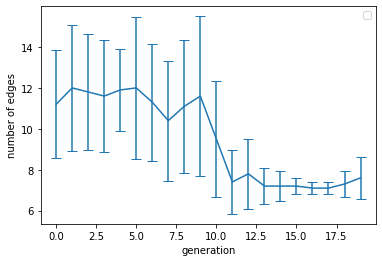
\includegraphics[clip,width=75mm]{edge.png}
    \caption{世代ごとのショートカット数}
    \label{fig:edge}
  \end{center}
\end{figure}

\begin{figure*}[tb]
 \begin{minipage}{0.5\hsize}
 	\begin{center}
 		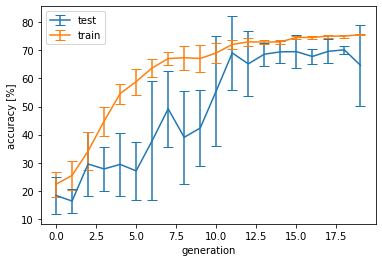
\includegraphics[clip,width=75mm]{acc.png}
 		\caption{世代ごとの精度 (平均と標準偏差)}
 		\label{fig:acc}
 	\end{center}
 \end{minipage}
 \begin{minipage}{0.5\hsize}
 	\begin{center}
 		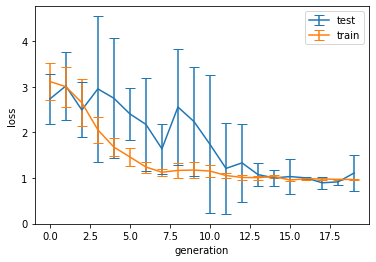
\includegraphics[clip,width=75mm]{loss.png}
 		\caption{世代ごとのロス (平均と標準偏差)}
 		\label{fig:loss}
 	\end{center}
 \end{minipage}
\end{figure*}

\begin{figure*}[tb]
 \begin{minipage}{0.5\hsize}
 	\begin{center}
 		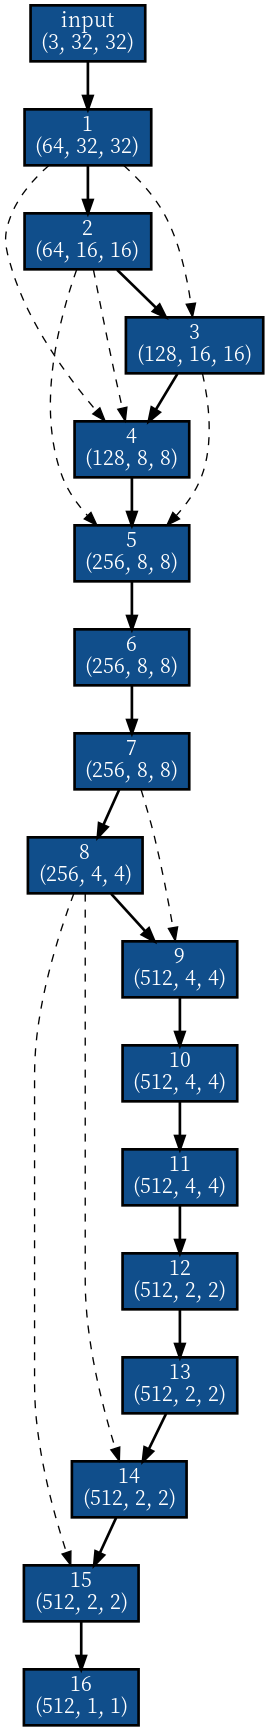
\includegraphics[clip,scale=0.25]{graph_g1.png}
 		\caption{1世代目の最良個体}
 		\label{fig:graph1}
 	\end{center}
 \end{minipage}
 \begin{minipage}{0.5\hsize}
 	\begin{center}
 		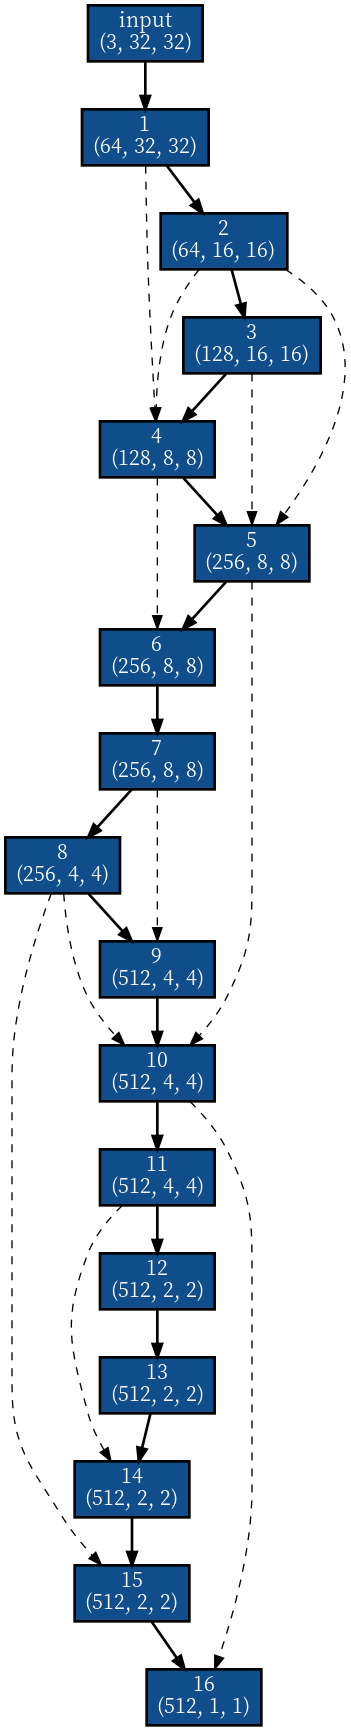
\includegraphics[clip,scale=0.25]{graph_g20.png}
 		\caption{20世代目の最良個体}
 		\label{fig:graph20}
 	\end{center}
 \end{minipage}
\end{figure*}

\section{今後の予定}
% なんとなくなんかの勉強をするとかではなく具体的に

来週は発表の資料を作成する.

sshのエラーに実験を中断されられたが, 次回はこれを修正してさらに大規模に実験する.

\begin{lstlisting}[caption=error log,label=code]
client_loop: send disconnect: Connection reset by peer
\end{lstlisting}


\section{ソースコード}
% 埋め込みでもGitでもいいので参照できるように
githubのnotebookリポジトリ参照.

% 参考文献リスト
\bibliographystyle{unsrt}
\bibliography{ref}
\end{document}
